\renewcommand{\LifeChapter}{y}
\chapter{Introduction}
\label{chap:introduction}

\chaptertoc{}

\begin{chapterabstract}
  This purpose of this chapter is to introduce the main motivations behind this project, from the historical relevance of \acl{dMRI} to the use of modern simulations for validating and developing new \acl{dMRI} models.
  This chapter also sets out the problem that this project aims to address and the specific aims for addressing various aspects of it.
\end{chapterabstract}

\section{Motivation}
\label{sec:intro_motivation}
In 1992, James Watson, co-discoverer of DNA, said ``The brain is the last and grandest biological frontier, the most complex thing we have yet discovered in our universe.''\cite{NAP1785}.
One year later, Francis Crick, fellow discoverer of DNA, and Edward Jones published a commentary in Nature lamenting how little was understood about human neuroanatomy, saying that new techniques were needed beyond the contemporary tracer studies in non-human primates \cite{Crick1993}.\footnote{This introduction was inspired by Richard Passingham's very nice foreword to Diffusion MRI by Berg and Behrens \cite{Johansen-Berg2013}}

Just one year after that, in 1994, Basser et al.\ \cite{Basser1994} showed that it was possible to use \ac{MRI} to measure the movement of water along axons, providing the basis for exactly the kind of new technique Crick and Jones had felt was needed.
This technique of using \ac{MRI} for measuring the movement of water molecules is known as \ac{dMRI}.

In the 25 years since the work of Basser et al., \acl{dMRI} has grown into a major \ac{MRI} research field, generating thousands of publications per year.
Diffusion MRI has found extensive use for imaging the brain, generating new techniques such as tractography, which attempts to map out the connections in the brain \emph{in vivo}, and microstructure imaging, in which measurements of the diffusion of water in tissue are used to infer information about the structure of the tissue on a scale much lower than the size of an MRI voxel.

\begin{comment}
\ac{MRI} provides researchers and clinicians a powerful and flexible tool for non-invasively imaging the human body \emph{in vivo} and has found extensive use over the past few decades in furthering the understanding the structure and function of the human brain.
One technique which is commonly employed to study the structure of the human brain is \ac{dMRI}.
\end{comment}

These techniques work because \ac{dMRI} sensitises the \ac{MRI} signal to the diffusive motion of water molecules on the micrometer scale - the further the water diffuses, the more strongly the MR signal is attenuated.
The environment in which the water molecules move restricts the motion of the molecules and so will affect how strongly the \ac{dMRI} signal is attenuated.
This dependency of the \ac{dMRI} signal on the environment in which water molecules diffuse can be exploited to infer information about the environment solely from the \ac{dMRI} signal.  

Microstructure imaging attempts to do exactly this, infer information about the microstructural environment such as cell size and density from the \ac{dMRI} signal.
Since the microstructural environment is on a much smaller scale than the \ac{dMRI} voxels, we cannot directly image this structure, so models are used to relate the \ac{dMRI} signal from a voxel to microstructural features.

The validation of these microstructural models can be difficult since ground truth microstructural features are typically inaccessible \emph{in vivo} and classical histological validation techniques have limitations such as disruption due to tissue extraction and preparation.

One approach commonly taken for the validation of new models is simulation of the \ac{dMRI} signal using well defined and controllable ground truth microstructural environments known as numerical phantoms which allow us to compare model fitting results to the ground truth from the numerical phantoms. Recent studies have used this approach to investigate grey matter \cite{Palombo2020}, however numerical phantoms have more commonly been used to study \ac{dMRI} in \ac{WM} \cite{Li2019,Jelescu2017,Nilsson2017,Scherrer2016,Tariq2016,Daducci2015,Xu2014,Zhang2012,Nilsson2010}.

Another application of numerical phantoms which is growing in popularity is in the direct computational modelling of microstructure.
These techniques use machine learning or fingerprinting-style techniques to match simulated signals and the corresponding ground truth microstructure of the numerical phantom to the measured signal in order to directly estimate microstructural features without using and explicit analytical model \cite{Rensonnet2018,Hill2019,Palombo2018a,Nedjati-Gilani2017}.

As well as affecting the dMRI signal, tissue microstructure also affects other MR techniques such as susceptibility-weighted imaging \cite{Li2012,Lee2010}. For instance, simulations have been used to show that using realistic \ac{WM} axonal models affect the susceptibility weighted MR image differently to the commonly assumed straight cylinders \cite{Xu2018}.
It is, therefore, important to the MRI community to generate realistic \ac{WM} numerical phantoms which accurately capture microstructural features in order to get realistic simulated signal.

Typically, however, there is a mismatch between the true complexity of brain tissue and the numerical phantoms that are used in simulations, outlined in \Cref{fig:intro_overview}.
For instance, \ac{WM} fibres are commonly represented using simple geometric constructs such as straight, parallel cylinders \cite{Nilsson2010,Fieremans2010,Nilsson2009,Ford1997,Hall2009,Alexander2010}. Real \ac{WM} fibres, however, have complex shapes with morphological features such as undulation and diameter variation, as revealed by \ac{EM} studies \cite{Abdollahzadeh2019, Lee2019b}.

It is very difficult to know exactly how this complex microstructure impacts on the \ac{dMRI} signal and to understand which of these complex morphological features can be detected using \ac{dMRI}.
Developing new numerical phantoms which allow us to generate realistic \ac{WM} microstructure would enable us to study these effects with more control and detail as well as enabling us to validate new and existing \ac{dMRI} microstructure models more comprehensively.

Additionally, realistic \ac{WM} numerical phantoms would enable us to drive forward a new generation of computational models of \ac{WM}, using machine learning to link simulated signals to the realistic \ac{WM} microstructure which could potentially improve the accuracy of microstructure models. For instance, it may be possible to disentangle axonal loss and demyelination using these computational models which can give us valuable information for differential diagnosis in diseases such as \ac{MS}.

The first step on the road to developing these new computational models, however, is to develop a method to generate realistic \ac{WM} numerical phantoms with controllable microstructure. That is the main purpose of the work presented in this thesis, the development of a new tool to generate more realistic \ac{WM} numerical phantoms than was previously possible.
% order to validate models in scenarios that are as close as possible to \emph{in vivo} conditions, the realism of numerical phantoms should be improved, attempting to fully capture all of the microstructural variation found in \emph{in vivo}.


\begin{figure}
  \centering
  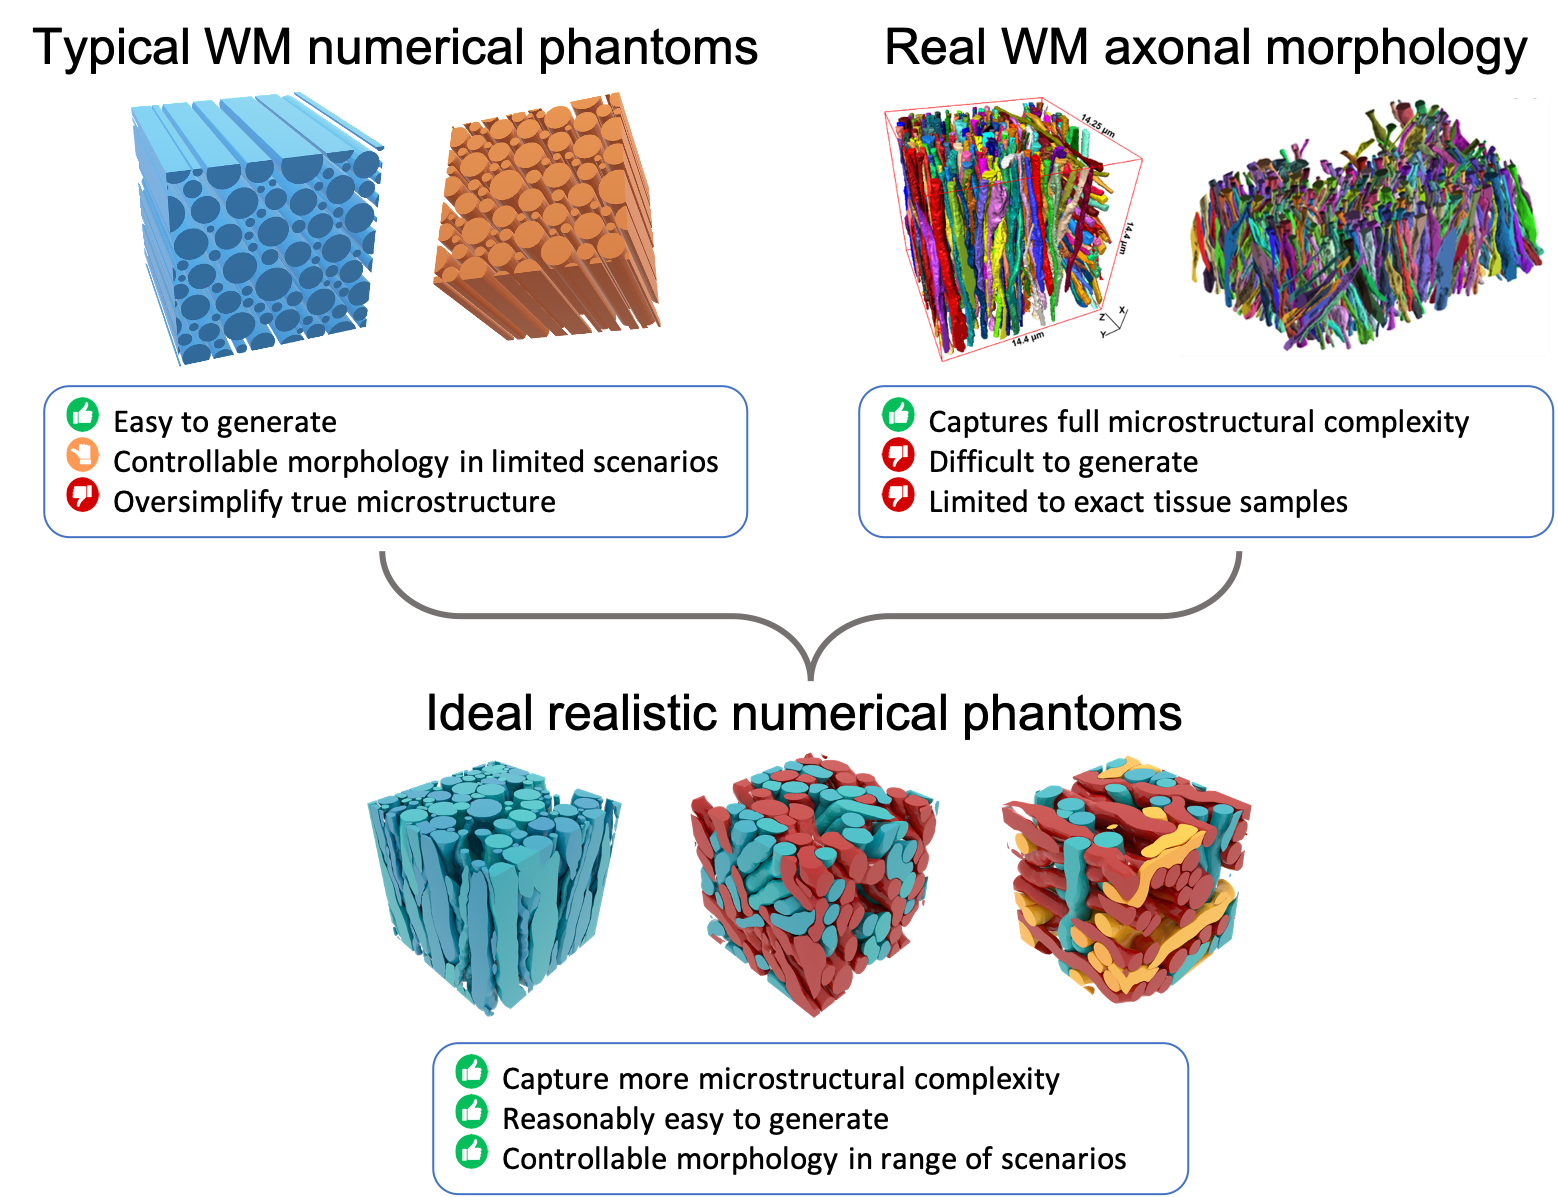
\includegraphics[width=\textwidth]{figures/introduction/overview}
  \caption[Overview of the main goal of the thesis]{The work presented in this abstract aims to bridge the gap between the true complexity of white matter axonal morphology and the simplistic representation currently used as numerical phantoms. }
  \label{fig:intro_overview}
\end{figure}

\section{Problem Statement}
\label{sec:intro_problem_statement}
There is a need to be able to generate numerical phantoms that realistically represent \ac{WM} microstructure, with controllable microstructural parameters such as axon packing density and orientation dispersion.


\section{Project Aims and Scope}
\label{sec:intro_project_aims}
This report summarises work towards improving the realism of simulations of diffusion \ac{MRI}. Realistic simulations allow models of the MRI signal to be validated using controllable and well known ground truth.

 

The mains aims of this work are as follows:
\begin{enumerate}
\item Develop a method for generating realistic \ac{WM} numerical phantoms with realistic and controllable morphology including axon packing densities and orientation dispersion
\item Test the realism of these numerical phantoms by comparing microstructure with real microstructure reconstructed from \acl{EM} and by comparing simulated \ac{dMRI} signal to real \ac{dMRI} signals from \ac{WM}
\item Use \ac{WM} numerical phantoms to probe assumptions in spherical deconvolution based dMRI modelling techniques.
\end{enumerate}

In an effort to achieve these aims, a method called\acused{ConFiG} \acs{ConFiG} (\textbf{Con}textual \textbf{Fi}bre \textbf{G}rowth) is presented which `grows' fibres densely attempting to respect some morphological priors to generate realistic \ac{WM} numerical phantoms.
%\ac{ConFiG} is tested, using it to general phantoms with simple morphology that can be easily generated using other means to test its ability to replicate simple situations and explore the input parameter space.


\section{Report Overview}
\label{sec:intro_report_overview}
The rest of the report is arranged as follows: \Cref{chap:background} outlines some of the physics behind \acl{dMRI} and how we simulate it. \Cref{chap:literature_review} reviews current literature on \ac{dMRI} simulations.~\Cref{chap:ipmi-implementation} presents a preliminary method for generating realistic \ac{WM} numerical phantoms and demonstrates its performance in some simple situations. \Cref{chap:config} outlines improvements to the preliminary method presented in \Cref{chap:ipmi-implementation}, resulting in the full \ac{ConFiG} algorithm. \Cref{chap:microstructure_eval} presents a series of experiments which were performed using \ac{ConFiG} phantoms to test how realistic the microstructure generated is when compare to real axonal morphology. \Cref{chap:frf_experiment} presents an experiment demonstrating an application of ConFiG phantoms to probe assumptions made in spherical deconvolution base \ac{dMRI} techniques. \Cref{chap:conclusion} summarises the work with some concluding remarks.



%%% Local Variables:
%%% mode: latex
%%% TeX-master: "../main"
%%% End:
